
% Beamer template Università Cattolica del Sacro Cuore
% Created by Francesco Bianchi
% Fall 2018

% NB Compile with XeLaTeX!

\documentclass[11pt, xcolor=dvipsnames]{beamer}

\usetheme[numbering=fraction, progressbar=frametitle, sectionpage=none, block=fill]{metropolis}
% regular, smallcaps, allsmallcaps, allcaps

\fontdir[Fira Sans font/]

\usepackage{appendixnumberbeamer}
\usepackage{graphicx}
\graphicspath{{Images/}}
\usepackage{transparent}
\usepackage{float}
\usepackage{tikz}
\usepackage{verbatim}
\usepackage{booktabs}
\usepackage{hyperref}
\usepackage{fancyvrb}
\usepackage{subfigure}
\usepackage[all]{nowidow}
\widowpenalty=1000
\usepackage{listings}
\usepackage{xcolor}

\xdefinecolor{Rgreen}{RGB}{44,131,61} 
\xdefinecolor{Rblue}{RGB}{58,95,205}

% Setup for R code appareance
\lstset{
        language=R, % set programming language 
        basicstyle=\ttfamily\small, % basic font style 
        keywordstyle=\color{Rblue}, % keyword style 
        commentstyle=\color{Rgreen}, % comment style 
        %numbers=left, % display line numbers on the left side 
        numberstyle=\ttfamily\tiny, % use small line numbers 
        numbersep=6pt,% space between line numbers and code
        backgroundcolor=\color{black!5},
        tabsize=3, % sizes of tabs 
        showstringspaces=false, % do not replace spaces in strings by a certain character 
        	frame=single,
        captionpos=t, % positioning of the caption above 
        breaklines=true, % automatic line breaking 
        escapeinside={(*}{*)}, % escaping to LaTeX 
        fancyvrb=true, % verbatim code is typset by listings 
        extendedchars=false, % prohibit extended chars (chars of codes 128--255) 
        %literate={"}{{\texttt{"}}}1%{<-}{{$\leftarrow$}}1{<<-}{{$\twoheadleftarrow$}}1 
        %{~}{{$\sim$}}1{<=}{{$\le$}}1{>=}{{$\ge$}}1{!=}{{$\neq$}}1{^}{{$^\wedge$}}1,% item to replace, text, length of chars 
        alsoletter={abline, plot}, % becomes a letter
        alsoother={abs, log, exp, $}, % becomes other 
        otherkeywords={!=, $, \&, \%*\%, \%\%}, % other keywords 
        deletekeywords={c}, % remove keywords 
        rulecolor=\color{black},
        %firstnumber=last
        belowcaptionskip=5pt
}

\usepackage{textpos}
\usepackage{tcolorbox}
\definecolor{Cattolica-Blue}{RGB}{0,94,149}
\definecolor{Cattolica-Yellow}{RGB}{237,154,40}
\definecolor{Metropolis-background}{RGB}{250,250,250}

\setbeamercolor{frametitle}{fg=White, bg=Cattolica-Blue}
\setbeamercolor{title separator}{fg=Cattolica-Yellow}
\setbeamercolor{progress bar in head/foot}{fg=Cattolica-Yellow, bg=Metropolis-background}
\setbeamercolor{alerted text}{fg=Cattolica-Yellow}

\setbeamertemplate{title graphic}{
  \vbox to 0pt {
    \vspace*{.84\textheight}  % change the value as necessary
    \hfill \inserttitlegraphic \hspace*{0.0025\textwidth}%
  }
  \nointerlineskip
}

\addtobeamertemplate{frametitle}{}{%
\begin{textblock*}{100mm}(.87\textwidth,-0.96cm)

\includegraphics[height=1.2cm, width=2cm, keepaspectratio]{Logo-White.pdf}
\end{textblock*}}

\newcommand{\btVFill}{\vskip1pt plus 1fill}

% To add footer in all slides, comment the following line to cancel it.
\setbeamertemplate{frame footer}{Author | Course Name}

%%%%%%%% Thesis Dissertation | Presentation %%%%%%%%
%%%%%%%% Title page definition %%%%%%%%

\title{Main title} % \newline Main Title (Cont.)}
\subtitle{Course Name}
\author{Professor Name Surname \\ \small{\href{mailto: name.surname@unicatt.it}{name.surname@unicatt.it}}\bigskip \medskip}
\date{Milan, December 31, 2018 \bigskip \medskip}
\institute{Università Cattolica del Sacro Cuore \\ M.Sc. in \LaTeX \\ Academic Year 2018 $-$ 2019} 
% Use \today to add today date
%\institute{Università Cattolica del Sacro Cuore \\ B.Sc. in ******* \\ Academic Year 20** $-$ 20**}
\titlegraphic{
\includegraphics[width=0.30\textwidth]{Logo-Grey.pdf}}

%%%%%%%%  %%%%%%%%

\begin{document}

\maketitle

\setbeamertemplate{background canvas}[default]

\section{General Information}

\begin{frame}
\frametitle{What is Beamer?}
\centering
\begin{minipage}{0.75\linewidth}
\textit{Beamer is a LaTeX document class for creating slides for presentations.}
\end{minipage}
\begin{table}[]
\centering
\caption{Beamer vs PowerPoint comparison}
\label{my-label}
\begin{tabular}{@{}lcc@{}}
\toprule
\textbf{} & \textbf{Beamer} & \textbf{PowerPoint} \\ \midrule
Math & Excellent & Medium \\
Animations & Good & Basic \\
Interoparability & Excellent & Good \\
Hyper Linking & \multicolumn{1}{l}{Excellent} & Poor \\
Tipography & \multicolumn{1}{l}{Excellent} & Good \\ \bottomrule
\end{tabular}
\end{table}
\end{frame}


\begin{frame}
\frametitle{Theme Options}
Metropolis theme provides a number of options, which can be set using a key=value interface. \newline
\texttt{\textbackslash \alert{usetheme}[option1=value1, ...]\{metropolis\}} \medskip

A list of some options follows:
 \begin{columns}
	\begin{column}{0.5\textwidth}
   	\begin{itemize}
   		\item \texttt{titleformat}
   		\item \texttt{sectionpage}	
   	\end{itemize}
   	\end{column}
   	\begin{column}{0.5\textwidth}
   	\begin{itemize}
   		\item \texttt{background}
   		\item \texttt{progressbar} \bigskip
   	\end{itemize}
   	\end{column}
\end{columns}
Newer projectors support a widescreen format such as 16:10 or 16:9 (Beamer default is 4:3) to change it use
\texttt{\textbackslash documentclass[aspectratio=1610]\{beamer\}}
\end{frame}

\begin{frame}
\frametitle{Listings}
\begin{enumerate}
	\item The first item 
	\item The second item
	\begin{enumerate}
		\item Nested item 1
		\item Nested item 2
	\end{enumerate}
	\item The third item
	\begin{itemize}
		\item Unnumbered item
		\item Unnumbered item	
	\end{itemize}
\end{enumerate}
\end{frame}


\begin{frame}
\frametitle{Math Environment}
\textbf{Exercise 1}
\textit{Let $f$ be the function}
	\begin{equation}
		y = log_2(|x|) + \frac{1}{x} \cdot e^{-\frac{1}{2} \cdot x}
	\label{equation-1}
	\end{equation}
	\textit{Plot the function $f$ in the interval ($-4; 4$).}
\end{frame}

\begin{frame}[fragile]
\frametitle{Blocks}
\begin{Example}
	Inline math $y = log_2(|x|) + \frac{1}{x} \cdot e^{-\frac{1}{2} \cdot x}$
\end{Example}
\pause
\begin{definition}
The definition of asymptote is $\hdots$
\end{definition}
\pause
\begin{theorem}
	A global maximum point is $\hdots$ while a local maximum is $\hdots$
\end{theorem}
\end{frame}

\begin{frame}[fragile]
\frametitle{Coding}
If you want to include (\textsf{R}) code in your presentation, please add \texttt{\textbackslash begin\{frame\}[fragile]} at the beginning of the slide. \bigskip
\begin{lstlisting}
f <- function(x) log2(abs(x)) + (1/x) * exp(-1/2*x)

plot(f, -4, 4, main="Exercise 1 Plot")
abline(h=0.32, lty=2)
abline(v=0.0, lty=2)
\end{lstlisting} 
\end{frame}

\begin{frame}
\frametitle{Figures}
\bigskip
\begin{figure}
\centering
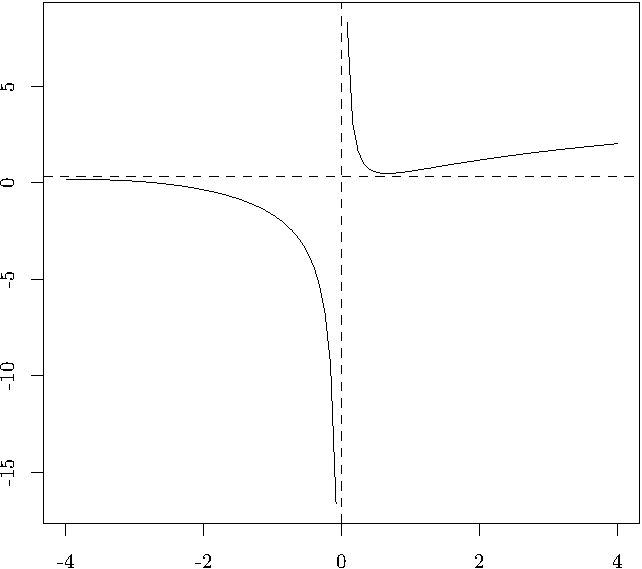
\includegraphics[width=0.6\textwidth]{Figure_1.pdf}
\caption{Exercise 1 plot}
\label{Exercise-1}	
\end{figure}
\end{frame}

%%%

%\appendix
\section{References}

\begin{frame}
\frametitle{References}
\small
%\scriptsize
\begin{enumerate}
\item[{[1]}] Bianchi F. (2018). \textit{"UCSC Dissertation Template"}. \href{https://github.com/Francesco-Bianchi/UCSC_dissertation_template}{GitHub}.
\item[{[2]}] Bianchi F. (2018). \textit{"UCSC Beamer Template"}. \href{https://github.com/Francesco-Bianchi/UCSC_beamer_template}{GitHub}.
\item[{[3]}] LaTeX team (2015). \textit{"LaTeX2e for authors"}. \href{https://www.latex-project.org/help/documentation/usrguide.pdf}{LaTeX Project}.
\end{enumerate}
\end{frame}

\end{document}
